
\section{Document Access Permission Control}
\label{s-accr}
The upload/download protocols of previous section do not launch until the gateway verifies that the requesting user has the proper permissions for accessing the external storage. There are two facets of the access permission verification problem. First, there must be a generic configuration mechanism for encoding the access control policy for associating and accessing external documents with the blockchain smart contracts of an application. Second, there must be an inviolable mechanism for enforcing the said access control policy in the storage integration gateway. Before we discuss these facets, we share our vision about the organization and relationship of the smart contracts of a blockchain application that set the requirements for document access control policy configuration.

\subsection{Blockchain Application Organization}
In our modeling, the smart contracts of a blockchain application form one or more rooted relationship hierarchies. The contracts deployed in the blockchain all come from a set of predefined contract templates and each deployed contract bears an application identifier and a type identifier that relate them to the owning application and the type template respectively.

For example, consider a blockchain application for crowd-funded real-estate assets development. The investors will receive ownership rights on parts of the asset. The asset developer will receive the profit for asset development. The actual development work will be conducted through a series of activities assigned to sub-contractors. In addition, some regulatory agency will be tagged with each asset development project by the local branch of the ministry of land for overseeing purposes. Finally, an investor can trade his/her share on the asset for profit. A probable contract template relationship hierarchy for this description can be as illustrated in Figure~\ref{fig-2}. It is apparent from the description that the root of the relationship in this case is the {\it Project} contract.
\begin{figure}[h]
\centering
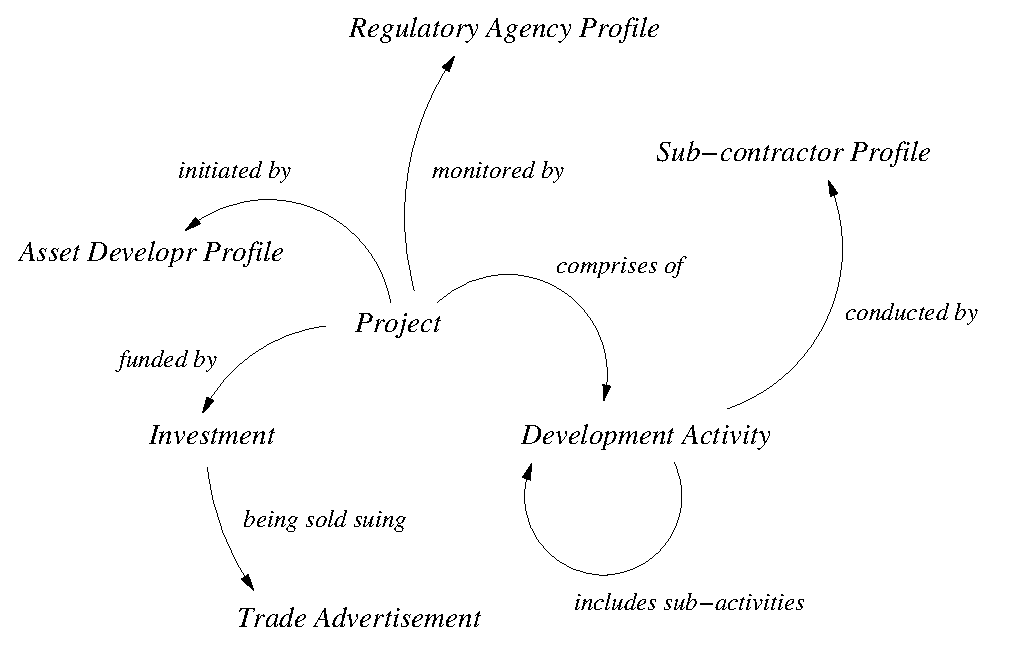
\includegraphics[width=0.48\textwidth]{access-req-example}                    
\caption{An example smart contract relationship hierarchy}\label{fig-2}
\end{figure}

Each contract in the hierarchy may have provision for associating external documents with it. Some of these documents will be public, i.e., accessible to any user upon submission of proper payment. For example, any would-be investor should be able to view documents related to project plan, and the profile of the asset developer and the regulatory agency to make an informed investment decision. Hence these documents should be public. Other documents will be protected and only accessible to users who are somehow related to the smart contracts associated with the documents through the rooted contract relationship hierarchy. For example, once a user invests on a project, he/she will own an investment contract. Only then he/she can access the profile related documents of all the sub-contractors who carry the string of of activities for that asset development project and any descriptive documents associated with those activities. However, he/she should not be able to view documents related to the payment negotiated between an assigner of activity and the assignee. Only the involved parties should see these documents. A regulatory agency representative should be able to view all documents associated with the project for proper supervision.    

For associating a document with a smart contract, i.e. document upload, the user must have direct access to the smart contract. For example, only the {\it owner} of an asset developer profile contract should be able to upload profile related documents and link them with his/her contract. He/she should be able to link new documents with a project contract only if he/she is the {\it creator} of the project. Meanwhile, both the {\it assigner} of a development activity and the {\it assignee} can link new documents with the activity. Hence, although in all cases a user must have direct association with the underlying smart contracts, the specific attribute of a contract that relates the user to it naturally varies.   

The expectation is that the access control policy configuration mechanism can encode all the various restrictions for document upload and download. Furthermore, the configuration mechanism must be generic as the storage integration gateway is not application specific and may be catering to the needs of multiple blockchain applications simultaneously. In other words, the gateway should not understand attributes such as {\it owner, creator,} and {assigner}; rather, it should interpret a common format of access control policy configuration and apply any configuration blindly.      
 
\subsection{Access Control Policy Configuration}
Our solution for generic specification of access control policies of various blockchain applications is to provide a simple language for expressing how a document bearer contract and the users allowed to access the document are related through the root of a contract relationship hierarchy. There are three components of each permission expression that grants a specific kind of users an specific kind of access to a specific document of a specific type of smart contract:
\begin{enumerate}
\item Source Linkage: a path description that tells how the root of the contract relationship hierarchy can be reached from the document bearer contract.
\item Accessor Linkage: another path description that tells how the root of the contract relationship hierarchy can be reached from the contract holding a reference of the user address.
\item Path Intersection Requirement: a specification that tells to what extent the source and accessor linkages should overlap to grant the user access to the document.     
\end{enumerate}            

\begin{figure*}[t!]
\footnotesize
\begin{bnf*}
\bnfprod{permission} {\bnfpn{docpermissions} \bnfor \bnfes}\\
\bnfprod{docpermissions}{\bnfpn{docpermission} \bnfor \bnfpn{docpermission} \bnfsp \bnfts{;} \bnfsp \bnfpn{docpermissions}}\\
\bnfprod{docpermission}{\bnfpn{doctype} \bnfsp \bnfpn{userpermissions}}\\
\bnfprod{userpermissions}{\bnfpn{userpermission} \bnfor \bnfpn{userpermission} \bnfsp \bnfts{AND} \bnfsp \bnfpn{userpermissions}}\\
\bnfprod{userpermission}{\bnfts{[} \bnfsp \bnfpn{permbits} \bnfsp \bnfts{]} \bnfsp \bnfpn{permexpr}}\\
\bnfprod{permexpr}{\bnfpn{localexpr} \bnfor \bnfpn{remoteexpr}}\\
\bnfprod{doctype}{\bnfpn{attrname} \bnfsp \bnfts{:} \bnfsp \bnfpn{attrmult} \bnfsp \bnfts{--}}\\
\bnfprod{permbits}{\bnfts{r-} \bnfor \bnfts{-w} \bnfor \bnfts{rw}}\\
\bnfprod{localexpr}{\bnfts{(} \bnfsp \bnfpn{attrname} \bnfsp \bnfts{:} \bnfsp \bnfpn{attrmult} \bnfsp \bnfts{)}}\\
\bnfprod{remoteexpr}{\bnfpn{acclink} \bnfsp \bnfts{/} \bnfsp \bnfpn{srclink} \bnfsp \bnfts{/} \bnfsp \bnfpn{overlap}}\\
\bnfprod{acclink}{\bnfts{accessor} \bnfsp \bnfts{(} \bnfpn{attrmult} \bnfsp \bnfts{)} \bnfsp \bnfts{[} \bnfpn{pathdirection} \bnfsp \bnfts{]} \bnfsp \bnfts{=} \bnfpn{path} \bnfsp \bnfts{=} \bnfsp \bnfts{root}}\\
\bnfprod{srclink}{\bnfts{this} \bnfsp \bnfts{=} \bnfsp \bnfpn{path} \bnfsp \bnfts{=} \bnfsp \bnfts{root}}\\
\bnfprod{overlap}{\bnfts{none} \bnfor \bnfts{substr}}\\
\bnfprod{pathdirection}{\bnfts{F} \bnfor \bnfts{R}}\\
\bnfprod{path}{\bnfpn{edge} \bnfor \bnfpn{edge} \bnfsp \bnfts{--} \bnfsp \bnfpn{path}}\\
\bnfprod{edge}{\bnfpn{linkerprop} \bnfsp \bnfts{:} \bnfsp \bnfpn{contracttype} \bnfsp\bnfpn{occurrences}}\\
\bnfprod{attrname}{\bnfpn{string}}\\
\bnfprod{attrmult}{\bnfts{single} \bnfor \bnfts{array}}\\
\bnfprod{linkerprop}{\bnfpn{string}}\\
\bnfprod{contracttype}{\bnfpn{string}}\\
\bnfprod{occurrences}{\bnfes \bnfor \bnfts{*}}
\end{bnf*}
\normalsize
\caption{Permission Expression Grammar}
\label{grammar}
\end{figure*}

Figure~\ref{grammar} describes the grammar for permission policy configuration for a document bearer smart contract. The grammar requires that access permissions are specified per document type and individually for each approved user category. For example, assume in the contract relationship hierarchy of Figure~\ref{fig-2}, the {\it investor} of any {\it Investment} contract, the {\it assigner} of an ancestor {\it DevActivity} contract, and any of the {\it representatives} of the {\it RegulatoryAgency} contract can view the {\it license} document of the {\it Subcontractor} contract corresponding to the {\it assignee} of a {\it DevActivity} of the underlying project. Meanwhile, only the {\it owner} of the {Subcontractor} contract can both read and replace (i.e., write) the {\it license} document in the external storage. Then the permission configuration for the {\it license} document should be as described in Listing~\ref{perm-ex}:

\lstset{caption=Example access permission configuration, label=perm-ex}
\lstinputlisting{permission-example.txt}

Our strategy for specifying the access permissions using contract relationship path expressions is a middle ground between access control list (ACL) and role based access control (RBAC) that are typically being used in file systems \cite{Barkley:1997:CSR:266741.266769}. Like RBAC, users gain access to resources because they held specific roles, due to their association with specific smart contracts. However, unlike generic roles in RBAC, these roles in our case are indirectly bound to specific resources through some relationship graphs.       

\subsection{Access Control Policy Enforcement}
A storage integration gateway does not need to understand smart contract relationship hierarchies to enforce access control rules specified in the permission expressions of various smart contracts. It only requires that the blockchain network notifies it whenever a smart contract is deployed. In addition, there are APIs to determine the template type of a deployed smart contract, to retrieve the permission expressions governing access to the documents associated with it, and to access metadata related to documents' locations in the external storage. Finally, contracts are required to emit properly formatted events\footnote{An event should contain the addresses of the two contracts whose direct association has been affected by the blockchain transaction, their template type names, and the nature of the update.} in response to blockchain transactions that may affect source or accessor linkages of various documents.\footnote{If we consider a smart contract relationship hierarchy as a directed graph, all relationships may not be traceable from the leaf to the root of the hierarchy. Some relationships may go backward from the root to the leave. Regardless, the events on the audit log should be formatted to support a uniform traversal strategy from the leave to the root.} All these are simple requirements that are easy to satisfy in any typical blockchain network supporting Ethereum Virtual Machine (EVM) specification for smart contracts \cite{Wood2014EthereumAS}.

The gateway monitors these events and derives a document permission database by combining event data and gateway's path expression related query results. This database is like a dynamic ACL database that is automatically being updated in response to new blockchain events. Figure~\ref{fig:perm-ERD} depicts a high level entity relationship diagram of the gateway's document database.
\begin{figure}[h]
\centering
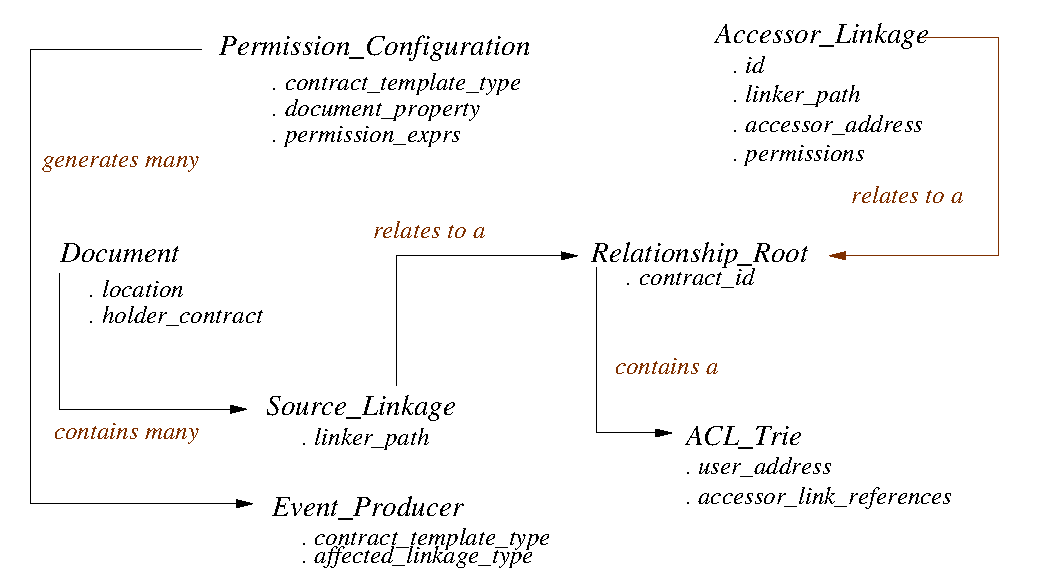
\includegraphics[width=0.48\textwidth]{permission-db}                    
\caption{Entity Relationship Diagram of the Access Permission Database}\label{fig:perm-ERD}
\end{figure}
       
As new smart contracts are being deployed in the blockchain network, the gateway updates contracts' template related information, if not already known, in local database to determine if a contract of this type can affect any document access permission through some source and accessor linkages. In addition, the gateway determines if this type of contract can be a root of any contract relationship hierarchy. For each contract that is a root of a contract relationship hierarchy, the gateway creates an ACL holding Markle tree (or trie) \cite{6233691} that contains the user addresses that are the endpoints of various accessor linkages originated from the root contract.

If a document is uploaded or an event is published about a change in any property that contributes an edge to the document's paths to various relationship roots, new source linkages are being computed and stored in the database. At the same time, invalidated source linkages are being eliminated. Similarly, if any smart contract property that contributes an edge to users' accessor path to various relationship roots, valid accessor linkages are being recomputed. In addition, the ACL tree entries of the affected users are also being updated.

When a user requests the gateway to undertake an upload/download protocol with the user, the gateway receives the underlying document bearing smart contract's address, the attribute of the smart contract the document refers to, and the user address. Since in case of an upload, the user must be associated with the document bearing smart contract directly, the gateway merely checks the smart contract template description to determine what query to issue in the smart contract to search for the user address. If the requesting user is found registered as a valid uploader then the upload protocol is initiated. Once upload is done, blockchain audit log is traversed to determine new source linkages for that document to existing contract relationship roots. This source linkages are then inserted in the gateway database. If the new document replaces some previously uploaded document then only the location related metadata need to be updated in the gateway database to point to the new document.       

If the user requests for a document download session, the gateway first identifies the ACL trees correspond to smart contract relationship roots reachable by traversing the source linkages of the document. Then it checks if the user's address exists in any of those ACL trees. Then it retrieves all accessor linkages ending at the user address in various ACL trees. Finally, related document source and accessor linkages are compared to decide if they can be combined satisfying any read permission configuration for the document. If any combination attempt succeeds then the user is granted access. If the authorization process fails in any of these steps then the user's request is denied.          
        
Note that although both upload and download protocol initialization request authorization involve local database lookups in the external storage integration gateway, the gateway can be arbitrarily replicated and each replica can resume afresh after a database crash because all information in a gateway database is derived from blockchain ledger data, thus easily recoverable.          
             
